\documentclass[a4paper,
fontsize=11pt,
%headings=small,
oneside,
numbers=noperiodatend,
parskip=half-,
bibliography=totoc,
final
]{scrartcl}

\usepackage[babel]{csquotes}
\usepackage{synttree}
\usepackage{graphicx}
\setkeys{Gin}{width=.4\textwidth} %default pics size

\graphicspath{{./plots/}}
\usepackage[ngerman]{babel}
\usepackage[T1]{fontenc}
%\usepackage{amsmath}
\usepackage[utf8x]{inputenc}
\usepackage [hyphens]{url}
\usepackage{booktabs} 
\usepackage[left=2.4cm,right=2.4cm,top=2.3cm,bottom=2cm,includeheadfoot]{geometry}
\usepackage[labelformat=empty]{caption} % option 'labelformat=empty]' to surpress adding "Abbildung 1:" or "Figure 1" before each caption / use parameter '\captionsetup{labelformat=empty}' instead to change this for just one caption
\usepackage{eurosym}
\usepackage{multirow}
\usepackage[ngerman]{varioref}
\setcapindent{1em}
\renewcommand{\labelitemi}{--}
\usepackage{paralist}
\usepackage{pdfpages}
\usepackage{lscape}
\usepackage{float}
\usepackage{acronym}
\usepackage{eurosym}
\usepackage{longtable,lscape}
\usepackage{mathpazo}
\usepackage[normalem]{ulem} %emphasize weiterhin kursiv
\usepackage[flushmargin,ragged]{footmisc} % left align footnote
\usepackage{ccicons} 
\setcapindent{0pt} % no indentation in captions
\usepackage{xurl} % Breaks URLs

%%%% fancy LIBREAS URL color 
\usepackage{xcolor}
\definecolor{libreas}{RGB}{112,0,0}

\usepackage{listings}

\urlstyle{same}  % don't use monospace font for urls

\usepackage[fleqn]{amsmath}

%adjust fontsize for part

\usepackage{sectsty}
\partfont{\large}

%Das BibTeX-Zeichen mit \BibTeX setzen:
\def\symbol#1{\char #1\relax}
\def\bsl{{\tt\symbol{'134}}}
\def\BibTeX{{\rm B\kern-.05em{\sc i\kern-.025em b}\kern-.08em
    T\kern-.1667em\lower.7ex\hbox{E}\kern-.125emX}}

\usepackage{fancyhdr}
\fancyhf{}
\pagestyle{fancyplain}
\fancyhead[R]{\thepage}

% make sure bookmarks are created eventough sections are not numbered!
% uncommend if sections are numbered (bookmarks created by default)
\makeatletter
\renewcommand\@seccntformat[1]{}
\makeatother

% typo setup
\clubpenalty = 10000
\widowpenalty = 10000
\displaywidowpenalty = 10000

\usepackage{hyperxmp}
\usepackage[colorlinks, linkcolor=black,citecolor=black, urlcolor=libreas,
breaklinks= true,bookmarks=true,bookmarksopen = true]{hyperref}
\usepackage{breakurl}

%meta
%meta

\fancyhead[L]{S. Franz \& M. Kindling\\ %author
LIBREAS. Library Ideas, 47 (2025). % journal, issue, volume.
\href{https://doi.org/10.18452/x}{\color{black}https://doi.org/10.18452/x}
{}} % doi 
\fancyhead[R]{\thepage} %page number
\fancyfoot[L] {\ccLogo \ccAttribution\ \href{https://creativecommons.org/licenses/by/4.0/}{\color{black}Creative Commons BY 4.0}}  %licence
\fancyfoot[R] {ISSN: 1860-7950}

\title{\LARGE{Offene Wissenschaft kartieren. Status quo von Open-Access-Strategien und Infrastrukturangeboten an deutschen Universitäten und Hochschulen im oa.atlas}}% title
\author{Simone Franz, Maxi Kindling} % author

\setcounter{page}{1}

\hypersetup{%
      pdftitle={Offene Wissenschaft kartieren. Status quo von Open-Access-Strategien und Infrastrukturangeboten an deutschen Universitäten und Hochschulen im oa.atlas},
      pdfauthor={Simone Franz, Maxi Kindling},
      pdfsubject={LIBREAS. Library Ideas, 47 (2025)},
      pdfkeywords={Open Access, oa.atlas, Deutschland, Bestandsaufnahme, Kartierung},
      pdflicenseurl={https://creativecommons.org/licenses/by/4.0/},
      pdfcopyright={CC BY 4.0 International},
      pdfcontacturl={http://libreas.eu},
      pdfurl={},
      pdfdoi={},
      pdflang={de},
      pdfmetalang={de}
     }



\date{}
\begin{document}

\maketitle
\thispagestyle{fancyplain} 

%abstracts
\begin{abstract}
\noindent
\textbf{Zusammenfassung}: Der Beitrag stellt das Angebot des oa.atlas
vor und bietet anhand von vier exemplarischen Kategorien Einblicke in
den Stand von Open Access an deutschen Universitäten und Hochschulen.

\begin{center}\rule{0.5\linewidth}{0.5pt}\end{center}

\noindent
\textbf{Abstract}: The article introduces the oa.atlas service and
illustrates the status of Open Access at German universities and higher
education institutions using four exemplary categories.
\end{abstract}

%body
\section{Was ist der oa.atlas?}\label{was-ist-der-oa.atlas}

Der oa.atlas ist eine laufend aktualisierte Datensammlung, die derzeit
im Rahmen des BMBF-geförderten Projekts open-access.network
bereitgestellt wird.\footnote{\url{https://open-access.network/startseite};
  künftig werden die Services des Projekts durch den Verein
  open-access.netwok e.\,V. in ein community-betriebenes Angebot
  überführt: \url{https://open-access.network/ueber-uns/verein}.} Das
Open Research Office Berlin (OROB) hat bereits im Jahr 2020 mit der
Konzeptionierung und Erfassung von Daten im Rahmen des oa.atlas
begonnen, um Strategien, Services und Maßnahmen rund um die
Open-Access-Transformation auf Ebene der Bundesländer\footnote{Übersicht
  nach deutschen Bundesländern siehe
  \url{https://oabb.pubpub.org/dash/collection/oa-atlas/overview}} und
der wissenschaftlichen Institutionen in Deutschland zu erfassen. Seit
2023 unterstützt der Projektpartner Helmholtz Open Science Office bei
der Kuratierung der Daten zu den Institutionen. Der Status quo
Open-Access- und Open-Science-bezogener Aktivitäten auf Ebene der
Institutionen in Deutschland wird im oa.atlas als Karten-, Listen- und
Detailansicht über das Portal open-access.network abgebildet.\footnote{\url{https://open-access.network/services/oaatlas}}
Weitere Informationen zum oa.atlas finden sich unter anderem in einem
Konzeptpapier (Kindling et al.~2024). Die Datensammlung des oa.atlas
kann zur freien Nutzung abgerufen werden.\footnote{\url{https://open-access.network/services/oaatlas/oaatlas-review}}
Derzeit wird eine Schnittstelle zur automatisierten Datenabfrage
vorbereitet.

Die Daten des oa.atlas können verwendet werden, um beispielsweise die
Verbreitung von Strategien und Maßnahmen auf der Ebene von einzelnen
Organisationen, Organisationstypen oder Bundesländern zu analysieren. In
diesem Beitrag wird das exemplarisch anhand einiger ausgewählter
Open-Access-bezogener Variablen demonstriert. Diese umfassen sowohl
(hochschul-) politische Strategien und Maßnahmen, zu denen sowohl die
Unterzeichnung der \emph{Berliner Erklärung über den offenen Zugang zu
wissenschaftlichem Wissen}, die Verabschiedung von Open Access Policies
und die Benennung von Open-Access-Beauftragten gehören, als auch
Infrastrukturangebote wie Repositorien, Open-Access-Verlage und
-Hostingdienste. Am Beispiel eines Datenabzugs von Dezember 2024 zeigt
dieser Beitrag Auswertungs- und Anknüpfungsmöglichkeiten für
weiterführende Fragestellungen.

\section{Welche wissenschaftlichen Institutionen werden hier
betrachtet?}\label{welche-wissenschaftlichen-institutionen-werden-hier-betrachtet}

Die nachfolgenden Analysen beziehen sich auf öffentliche Universitäten
und Hochschulen in Deutschland. Mit Stand 13. Dezember 2024 waren 101
Universitäten und 212 Hochschulen in öffentlich-rechtlicher oder
staatlich anerkannter kirchlicher Trägerschaft erfasst. Die
Kategorisierung der hier betrachteten Institutionen und ihrer
Trägerschaft basiert auf dem Hochschulkompass der
Hochschulrektorenkonferenz (HRK).\footnote{\url{https://www.hochschulkompass.de/home.html}}
Unter Hochschulen werden (Fach-)Hochschulen für Angewandte
Wissenschaften (HAW), künstlerische Hochschulen, Hochschulen eigenen
Typs sowie Verwaltungshochschulen zusammengefasst. Zudem werden neben
Universitäten auch Universitätskliniken aufgenommen, die der
Hochschulkompass nicht separat erfasst. Sie wurden deshalb in dieser
Analyse nicht mit ausgewertet.

\section{\texorpdfstring{Wie viele Universitäten und Hochschulen
haben die \emph{Berliner Erklärung über den offenen Zugang zu
wissenschaftlichem Wissen}
unterzeichnet?}{Wie viele Universitäten und Hochschulen haben die Berliner Erklärung über den offenen Zugang zu wissenschaftlichem Wissen unterzeichnet?}}\label{wie-viele-universituxe4ten-und-hochschulen-haben-die-berliner-erkluxe4rung-uxfcber-den-offenen-zugang-zu-wissenschaftlichem-wissen-unterzeichnet}

Die \emph{Berliner Erklärung über den offenen Zugang zu
wissenschaftlichem Wissen} (kurz: \emph{Berliner Erklärung}) vom 22.
Oktober 2003\footnote{\url{https://openaccess.mpg.de/Berliner-Erklaerung}}
gilt als einer der Meilensteine der Open-Access-Bewegung und wurde
inzwischen von über 800 Forschungsorganisationen und -institutionen
weltweit unterzeichnet. Diese verpflichten sich, die Umsetzung des
Open-Access-Gedankens zu unterstützen. Eine Auswertung des prozentualen
Anteils der Universitäten und Hochschulen in Deutschland zeigt, dass die
\emph{Berliner Erklärung} von weniger als der Hälfte der Einrichtungen
unterzeichnet wurde. Bei den Universitäten haben über 43 Prozent die Berliner Erklärung unterzeichnet, während es bei den Hochschulen nur etwas über 13 Prozent sind.

\begin{figure}[H]
\centering
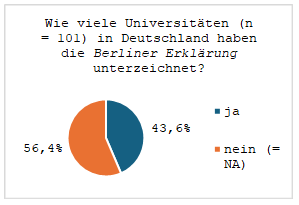
\includegraphics[]{img/image002.png}
\caption{Abbildung 1: Prozentualer Anteil der Universitäten (n = 101), welche die \emph{Berliner Erklärung} unterzeichneten}
\end{figure}

\begin{figure}[H]
\centering
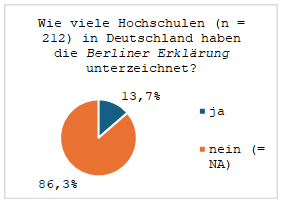
\includegraphics[]{img/image001.png}
\caption{Abbildung 2: Prozentualer Anteil der Hochschulen (n = 212), welche die \emph{Berliner Erklärung} unterzeichneten}
\end{figure}

Die Universität Kassel war 2004 die erste, welche die \emph{Berliner
Erklärung} unterschrieb. Eine Längsschnittanalyse in Abbildung 3 zeigt,
dass die Anzahl der unterzeichnenden Universitäten ab 2012 weiter
zunimmt (n = 5), was auf die nach wie vor anhaltende Bedeutung der
\emph{Berliner Erklärung} hindeutet. Die meisten Universitäten
unterzeichneten in den Jahren 2015 und 2016 (jeweils n = 8). Mit einigen
Jahren Verzögerung zogen auch die Hochschulen nach. Während die
Technische Hochschule (TH) Wildau 2007 Vorreiterin war, kamen erst ab
2021 (n = 6) und 2022 (n = 10) vergleichsweise viele Hochschulen hinzu.
Sowohl für Universitäten als auch für Hochschulen lässt sich nach wie
vor ein leicht steigender Trend beobachten, welcher die bleibende Bedeutung der \emph{Berliner Erklärung} auch nach 20
Jahren noch unterstreicht.

\begin{figure}[H]
\centering
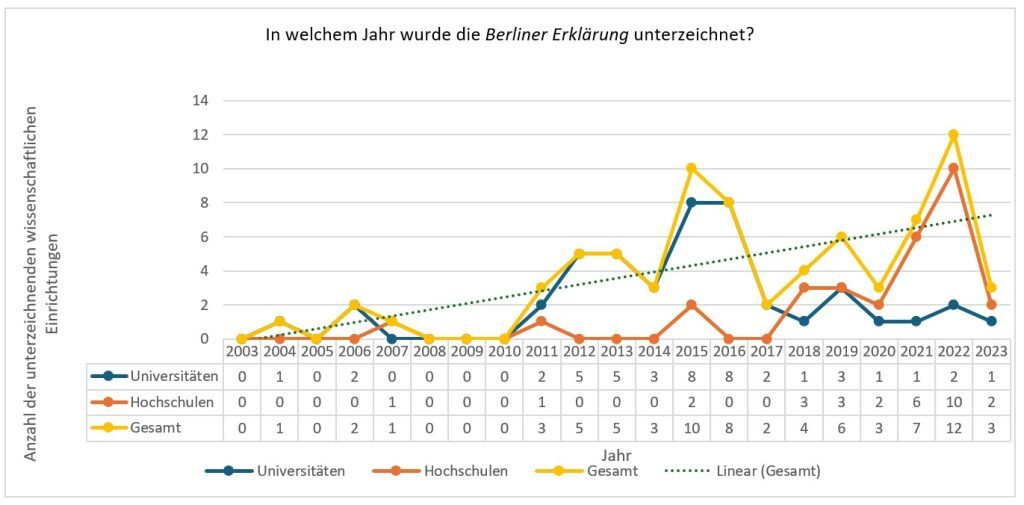
\includegraphics[width=1\textwidth]{img/image003.jpg}
\caption{Abbildung 3: Längsschnittanalyse zur Unterzeichnung der Berliner Erklärung für den Zeitraum 2003 bis 2023 an Universitäten (n = 101) und Hochschulen (n = 212)}
\end{figure}

\section{Wie viele Universitäten und Hochschulen verfügen über
eine Open Access
Policy?}\label{wie-viele-universituxe4ten-und-hochschulen-verfuxfcgen-uxfcber-eine-open-access-policy}

Als Open Access Policy definiert der oa.atlas eine von Gremien oder
Leitungsebenen verabschiedete Richtlinie, welche Rollen, Rechte und
Verantwortlichkeiten verschiedener Akteur*innen einer Institution für
die Umsetzung von Open Access empfiehlt.\footnote{Kurzbeschreibung der
  im oa.atlas erfassten Daten siehe
  \url{https://open-access.network/services/oaatlas/ueber-den-oaatlas}}
Sie legt häufig einen Schwerpunkt auf den freien Zugang zu
wissenschaftlichen Textpublikationen. Während rund 20\,Prozent der
Hochschulen eine Open Access Policy haben, sind es bei den Universitäten
fast 68\,Pro\-zent.

\begin{figure}[H]
\centering
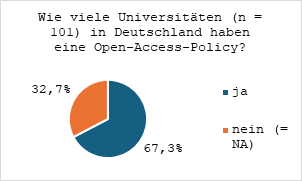
\includegraphics[]{img/image005.png}
\caption{Abbildung 4: Prozentualer Anteil der Universitäten (n = 101), die eine Open Access Policy verabschiedet haben}
\end{figure}

\begin{figure}[H]
\centering
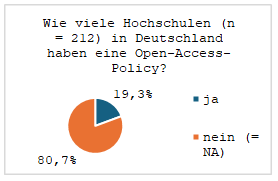
\includegraphics[]{img/image004.png}
\caption{Abbildung 5: Prozentualer Anteil der Hochschulen (n = 212), die eine Open Access Policy verabschiedet haben}
\end{figure}

Die in Abbildung 6 gezeigte Längsschnittanalyse unterstreicht, dass vor
allem ab 2011 die Zahl der verabschiedeten Open Access Policies an den
Universitäten sprunghaft ansteigt (n = 8) und ab 2019 (n = 3) abfällt. Dies
belegt, dass ab diesem Zeitpunkt verstärkt strukturbildende Maßnahmen an
den Einrichtungen umgesetzt wurden; hier besteht vermutlich unter
anderem ein Zusammenhang mit dem Programm \enquote{Open Access
Publizieren} der Deutschen Forschungsgemeinschaft (DFG), das den Aufbau
von Open-Access-Publikationsfonds an 45 deutschen Hochschulen zwischen
2010 und 2016 förderte (Ploder 2024). An den Hochschulen nimmt die Zahl
der verabschiedeten Policies in den Jahren 2018 (n = 10), 2020 (n = 7) und
2021 (n = 8) jeweils im Vergleich zu den Vorjahren zu. Seit 2021 fällt die
Kurve leicht ab. Im Jahr 2018 wurden sowohl bei den Universitäten als
auch bei den Hochschulen relativ viele Open Access Policies beschlossen
(insgesamt n = 19). In diesem Jahr hatten auch erstmals mehr Hochschulen
(n = 10) eine Open Access Policy als Universitäten (n = 9). So lässt sich
übergreifend für beide Institutionstypen ein leicht steigender Trend
erkennen. Während 2011, zwischen 2016 und 2018 sowie zwischen 2020 und
2022 die meisten Policies an Universitäten und Hochschulen verabschiedet
wurden, unterzeichneten Universitäten und Hochschulen die \emph{Berliner
Erklärung} 2015, 2016 und 2022 am häufigsten.

\begin{figure}[H]
\centering
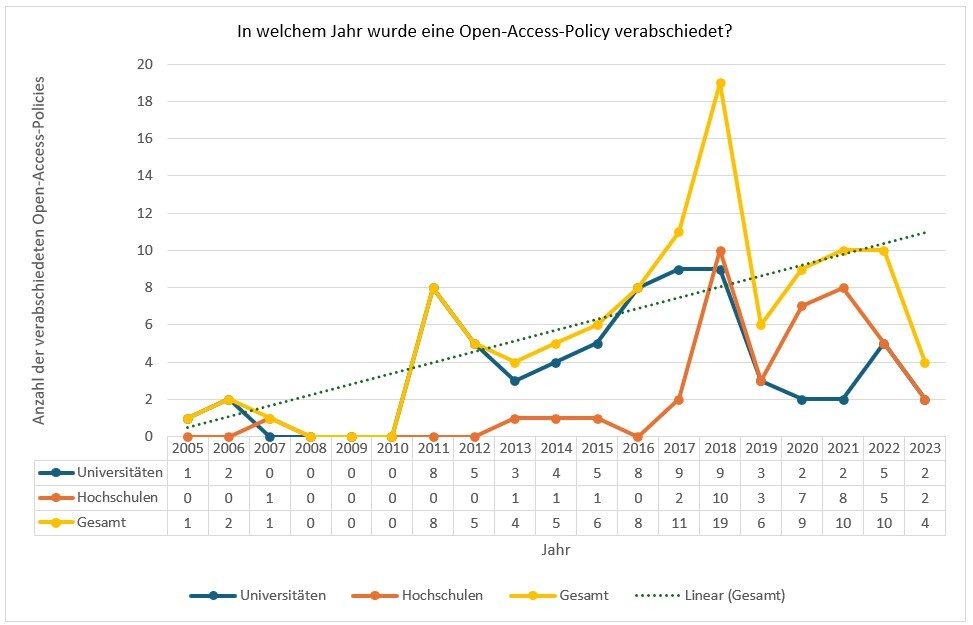
\includegraphics[width=1\textwidth]{img/image006.jpg}
\caption{Abbildung 6: Längsschnittanalyse zur Verabschiedung von Open Access Policies an Universitäten und Hochschulen (n = 212)}
\end{figure}

\section{Wie viele Universitäten und Hochschulen haben
Open-Access-Beauftragte
benannt?}\label{wie-viele-universituxe4ten-und-hochschulen-haben-open-access-beauftragte-benannt}

Open-Access-Beauftragte repräsentieren laut Definition des oa.atlas das
Thema Open Access inner- und außerhalb ihrer Institution beispielsweise
durch das Voranbringen strategischer Fragen. Von den Hochschulen haben
mit rund 7 Prozent relativ wenige solche Open-Access-Beauf\-tragte.
Auch die Universitäten haben nur zu knapp einem Drittel
Open-Access-Beauftragte benannt (36,6\,\%); die überwiegende Mehrheit von
89 Universitäten hat aber eine Ansprechperson für Open Access, die auf
der Website der Institution genannt wird. In einer tiefergehenden
Analyse könnte der Frage nachgegangen werden, ob es einen Zusammenhang
zwischen Open-Access-Beauftragen und Open Access Policies gibt. In jedem
Fall deutet sich eine Lücke an. Auf der einen Seite stehen die Policies
und die Unterzeichnung von Erklärungen, die zur Konsens- und
Community-Bildung beitragen sowie als Absichtserklärungen zum Teil auch
performativen Charakter haben. Auf der anderen Seite findet sich eine im
Vergleich eher zurückhaltende konkrete Implementierung und Umsetzung von
Maßnahmen in der Praxis durch offizielle Mandatsträger*innen wie
Open-Access-Beauftragte. Dabei gibt es regionale Unterschiede. So zeigt
der aktuelle Open-Access-Bericht für das Land Berlin, dass gemäß der
Vorgabe der Berliner Open-Access-Strategie von 2015 fast alle Berliner
Universitäten und Hochschulen Open-Access-Beauftragte benannt haben
(Kindling et al.~2024a).

\begin{figure}[H]
\centering
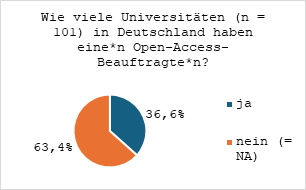
\includegraphics[]{img/image008.png}
\caption{Abbildung 7: Prozentualer Anteil der Universitäten (n = 101), die eine*n Open-Access-Beauftragte*n ernannt haben}
\end{figure}

\begin{figure}[H]
\centering
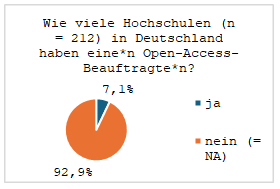
\includegraphics[]{img/image007.png}
\caption{Abbildung 8: Prozentualer Anteil der Hochschulen (n = 212), die eine*n Open-Access-Beauftragte*n ernannt haben}
\end{figure}

\section{Wie viele Universitäten und Hochschulen bieten ihren
Angehörigen Repositorien für die Veröffentlichung und Archivierung von
Publikationen?}\label{wie-viele-universituxe4ten-und-hochschulen-bieten-ihren-angehuxf6rigen-repositorien-fuxfcr-die-veruxf6ffentlichung-und-archivierung-von-publikationen}

Repositorien sind Dokumentenserver, die an Universitäten und
Forschungseinrichtungen betrieben und auf denen wissenschaftliche
Materialien archiviert sowie weltweit offen und langfristig zugänglich
gemacht werden. Publikationsinfrastrukturen in Form von Repositorien
sind Teil der wissenschaftseigenen, nicht-kommerziell ausgerichteten
Infrastruktur. Sie tragen dazu bei, die Souveränität über Daten zu
behalten und das Tracken von Forschenden durch kommerzielle \emph{Data
Analytics Business} zu unterbinden (Siems 2022).

Es zeigt sich, dass das Angebot von Repositorien insbesondere bei
Universitäten mit über 93\,Pro\-zent sehr weit verbreitet ist. Bei den
Hochschulen bieten etwas weniger als die Hälfte solche Services an
(48,6\,\%). Unter diesen sind auch kooperativ genutzte Angebote wie
beispielsweise ein durch die drei künstlerischen Hochschulen in Berlin
(Hochschule für Musik Hanns Eisler Berlin, Weißensee Kunsthochschule
Berlin, Hochschule für Schauspielkunst Ernst Busch) gemeinsam genutztes
Repositorium. In der Umsetzung von Open Access haben Repositorien als
institutionelle Infrastruktur, insbesondere für Zweitveröffentlichungen,
eine zentrale Funktion (Martin et al. 2023). Im besten Fall sind sie
DINI-zertifiziert (Oberländer 2017). Die im oa.atlas erfassten Daten
verdeutlichen, dass dies nur bei 52 der insgesamt 197 Repositorien der
Fall ist -- davon haben allerdings mit Erscheinen des DINI-Zertifikats 2025 40 ihre
Gültigkeit verloren.\footnote{Definition des oa.atlas: \enquote{Ein
  einmal ausgestelltes Zertifikat verliert mit der Veröffentlichung der
  dritten Nachfolgeversion des Kriterienkatalogs seine Gültigkeit.
  Derzeit gültige Versionen: 2016, 2019, 2022.}
  \url{https://open-access.network/services/oaatlas/ueber-den-oaatlas}. Im September 2025 wurde eine neue Version des Zertifikats veröffentlicht.}
Die noch gültig zertifizierten Repositorien verteilen sich auf die TH Wildau und Universitäten. Mit
Blick auf das Gesamtangebot an Repositorien zur Unterstützung des
Open-Access-Publizierens sollte die Bedeutung von
Publikationsinfrastrukturen über institutionelle Angebote hinaus nicht
außer Acht gelassen werden: So publizieren Forschende aus vielen
Bereichen der Natur- und Lebenswissenschaften auf Angeboten wie arXiv,
ChemRxiv, bioRxiv, medRxiv oder PubMed Central (PMC). Auch bestehen
disziplinübergreifende Ansätze wie beispielsweise das nationale
Repositorium HAL in Frankreich\footnote{\url{https://hal.science/}}, das
eine zentrale Komponente der Umsetzung der Open Science Policy
Frankreichs (\emph{National Plan for Open Science}) darstellt und unter
anderem von der französischen Regierung finanziert wird (Schöpfel et
al. 2024, S. 174). Ein solche Policy und damit verbundenes nationales
Angebot besteht hingegen in Deutschland nicht. Weiter untersuchenswert
wäre, ob eine stärkere Konsolidierung zu einer Entlastung personeller
und finanzieller Ressourcen führen kann (Brembs et al.~2021, 01:24:34--01:25:06) und inwieweit
eine verteilte und gut vernetzte Infrastruktur eine nachhaltig
ausgerichtete Landschaft an offenen Infrastrukturen stärken kann -- dazu
hat jüngst etwa die DFG ein Diskussionspapier veröffentlicht (DFG 2025).

\begin{figure}[H]
\centering
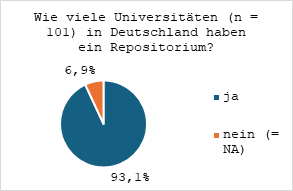
\includegraphics[]{img/image010.png}
\caption{Abbildung 9: Prozentualer Anteil der Universitäten (n = 101), die ein institutionelles Repositorium bereitstellen}
\end{figure}

\begin{figure}[H]
\centering
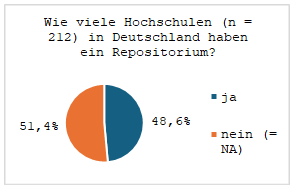
\includegraphics[]{img/image009.png}
\caption{Abbildung 10: Prozentualer Anteil der Hochschulen (n = 212), die ein institutionelles Repositorium bereitstellen}
\end{figure}

\section{Wie viele Universitäten und Hochschulen betreiben ein Hosting für Journals}\label{wie-viele-universituxe4ten-und-hochschulen-betreiben-open-access-verlage-undoder-hostingdienste-fuxfcr-zeitschriften}

Die im oa.atlas erfassten Open-Access-Verlage und Hostingdienste für Zeitschriften werden durch die Universitäten und die Hochschulen selbst betrieben. Die Daten im oa.atlas zeigen, dass bereits
mehr als ein Viertel aller Universitäten (25,7\,\%) über einen
Open-Access-Verlag \mbox{und/}oder Hostingdienste (37,6\,\%) verfügen. Dem
oa.atlas ist ebenso zu entnehmen, dass 18 Universitäten sowohl einen
Verlag als auch einen Hostingdienst betreiben. Im Fall von Berlin
Universities Publishing (BerlinUP), getragen von den Bibliotheken der
Freien Universität Berlin, der Humboldt-Universität zu Berlin, der
Technischen Universität Berlin und der Charité -- Universitätsmedizin
Berlin, erfolgt der Betrieb kooperativ.\footnote{\url{https://www.berlin-universities-publishing.de/}}
An Hochschulen sind Open-Access-Verlage (0,9\,\%) und Hostingdienste
(1,4\,\%) dagegen wohl unter anderem aufgrund des geringeren
Publikationsaufkommens und fehlender Open-Access-Strukturen kaum
vorhanden. Lediglich die Hochschule für Technik, Wirtschaft und Kultur
Leipzig (HTWK) hat einen eigenen Verlag, während die Hochschule für
Politik München (HfP) eine gemeinsame Infrastruktur mit dem Verlag der
Technischen Universität München (TUM) nutzt. Nur die Hochschule
Hannover, die Fachhochschule Münster und die Technische Hochschule
Würzburg-Schweinfurt (THWS) haben Instanzen zum Hosten von Journals.


\begin{figure}[H]
\centering
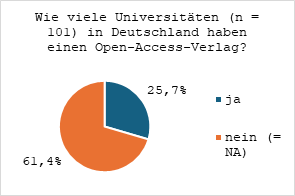
\includegraphics[]{img/image012.png}
\caption{Abbildung 11: Prozentualer Anteil der Universitäten (n = 101) mit Open-Access-Verlagen}
\end{figure}

\begin{figure}[H]
\centering
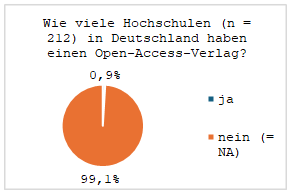
\includegraphics[]{img/image011.png}
\caption{Abbildung 12: Prozentualer Anteil der Hochschulen (n = 212) mit Open-Access-Verlagen}
\end{figure}

\begin{figure}[H]
\centering
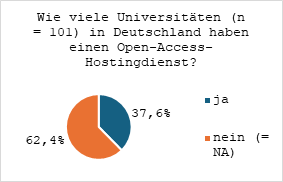
\includegraphics[]{img/image014.png}
\caption{Abbildung 13: Prozentualer Anteil der Universitäten (n = 101) mit Hostingdiensten}
\end{figure}

\begin{figure}[H]
\centering
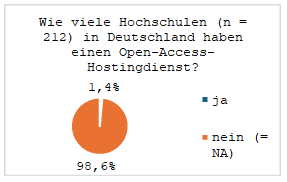
\includegraphics[]{img/image013.png}
\caption{Abbildung 14: Prozentualer Anteil der Hochschulen (n = 212) mit Hostingdiensten}
\end{figure}

Im Zuge des Ausbaus von Diamond-Open-Access-Angeboten an deutschen
Wissenschaftsinstitutionen ist zu erwarten, dass dem institutionellen
und durch die Wissenschaft getragenen Angebot von
Publikationsinfrastrukturen künftig eine noch größere Bedeutung zukommt.
Der weitere Ausbau wird sich auch anhand des oa.atlas nachzeichnen
lassen. Darüber hinaus zeigen die in diesem Beitrag betrachteten
Variablen nur einen Teil der über den oa.atlas möglichen Analysen.
Änderungswünsche zu den erfassten Informationen können über das
Review-Formular\footnote{\url{https://open-access.network/services/oaatlas/oaatlas-review}}
übermittelt werden. Allgemeines Feedback nimmt die Redaktion des
oa.atlas gerne entgegen.\footnote{\url{https://open-access.network/services/oaatlas}}

\section{Anmerkung}\label{anmerkung}

Bei diesem Beitrag handelt es sich um eine leicht überarbeitete Fassung
des Blogbeitrags der Autorinnen im Open Research Blog Berlin: Franz,
Simone \& Kindling, Maxi (2025) Offene Wissenschaft kartieren. Status
quo von Open-Access-Strategien und Infrastrukturangeboten an
Universitäten und Hochschulen im oa.atlas. DOI:
\url{https://doi.org/10.59350/6bhhc-f8j85}

\section{Referenzen}\label{referenzen}

Brembs, Björn; Degkwitz, Andreas; Holzer, Angela; Reda, Felix \& Wiarda,
Jan-Martin (2021) Wenn du nicht für das Produkt bezahlst, bist du
selbst das Produkt? Eine Podiumsdiskussion zur Kommerzialisierung von
Offener Wissenschaft. TIB AV-Portal. DOI:
\url{https://doi.org/10.5446/55690}

Deutsche Forschungsgemeinschaft (2025) Digitale Forschungspraxis und
kooperative Informationsinfrastrukturen. Ein Diskussionspapier der
Deutschen Forschungsgemeinschaft (DFG) zu Förderung und Finanzierung
wissenschaftlicher Informationsinfrastrukturen. DOI:
\url{https://doi.org/10.5281/zenodo.14621979}

Martin, Linda; Kindling, Maxi \& Rücknagel, Jesko (2023)
Zweitveröffentlichungsservices an Hochschulen. Bericht zur Erhebung
(1.0). DOI: \url{https://doi.org/10.5281/zenodo.7990619}

Kindling, Maxi; Neufend, Maike \& Fischer, Georg (2024a)
Organisationsentwicklung und Kompetenzvermittlung. In: Open-Access-Büro
Berlin et al.~(2024) Open-Access-Bericht Berlin. DOI:
\url{https://doi.org/10.21428/986c5d43.3ba47a23}

Kindling, Maxi; Martin, Linda \& Neufend, Maike (2024) oa.atlas:
Konzept. \emph{Open Research Office Berlin}. DOI:
\url{https://doi.org/10.21428/986c5d43.54fbd167}

Oberländer, Anja (2017) Förderung von Open Access über institutionelle
Infrastrukturen, insbesondere Repositorien. In: Söllner, Konstanze \&
Mittermaier, Bernhard {[}Hrsg.{]} Praxishandbuch Open Access. De
Gruyter Saur, S. 137--145. DOI:
\url{https://doi.org/10.1515/9783110494068-016}

Ploder, Michael et al.~(2020) Das DFG-Förderprogramm Open Access
Publizieren -- Bericht über die Förderung. Zenodo. DOI:
\url{https://doi.org/10.5281/zenodo.4486411}

Schöpfel, Joachim; Azeroual, Otmane; Chaudiron, Stéphane; Jacquemin,
Bernard; Kergosien, Eric; Prost, Hélène \& Thiault, Florence (2024) From
Open Repositories to CRIS -- A Case Study. In: Procedia Computer Science
249. DOI: \url{https://doi.org/10.1016/j.procs.2024.11.061}

Siems, Renke (2022) Das Lesen der Anderen: Die Auswirkungen von User
Tracking auf \mbox{Bibliotheken}. O-Bib. Das offene Bibliotheksjournal 9(1),
1--25. DOI: \url{https://doi.org/10.5282/o-bib/5797}

%autor
\begin{center}\rule{0.5\linewidth}{0.5pt}\end{center}

\textbf{Simone Franz} (\url{https://orcid.org/0000-0003-4525-6977}) ist
promovierte Frühneuzeithistorikerin und wissenschaftliche
Bibliothekarin. Derzeit ist sie wissenschaftliche Mitarbeiterin im
Bereich Publikationsdienste der Technischen Informationsbibliothek und
Datenmanagerin im Projekt \enquote{Prize Papers. Erschließung --
Digitalisierung -- Präsentation} (Niedersächsische Akademie der
Wissenschaften zu Göttingen/Carl von Ossietzky Universität Oldenburg,
Institut für Geschichte). Sie studierte Geschichte und Europäische
Ethnologie an der Humboldt-Universität zu Berlin sowie Archival Studies
und Niederlandistik an der Universiteit Leiden (Niederlande).

\textbf{Maxi Kindling} (\url{https://orcid.org/0000-0002-0167-0466}) ist promovierte Informationswissenschaftlerin und
leitet die Abteilung Publikationsdienste an der Universitätsbibliothek
der Technischen Universität Berlin. Zum Zeitpunkt der Arbeit mit dem
oa.atlas war sie Leiterin des Open-Access-Büros Berlin, einem von sechs
Projektpartnern im BMFTR-geförderten Projekt open-access.network.

\end{document}